\documentclass[10pt]{beamer}

\usepackage[spanish, mexico]{babel}
\usepackage[utf8]{inputenc}

\usetheme[progressbar=frametitle]{metropolis}
\usepackage{appendixnumberbeamer}

\usepackage{booktabs}
\usepackage[scale=2]{ccicons}

\usepackage{tikz}
\def\checkmark{\tikz\fill[scale=0.4](0,.35) -- (.25,0) -- (1,.7) -- (.25,.15) -- cycle;}
\usepackage{pgfplots}
\usepgfplotslibrary{dateplot}

\usepackage{xspace}
\newcommand{\themename}{\textbf{\textsc{metropolis}}\xspace}

%%
\usepackage{color}
\definecolor{lstgrey}{rgb}{0.95,0.95,0.95}
\definecolor{mygreen}{RGB}{28,172,0} % color values Red, Green, Blue
\definecolor{mylilas}{RGB}{170,55,241}

\usepackage{listings}
\lstset{language=Python,
       backgroundcolor=\color{lstgrey},
       frame=single,
       basicstyle=\footnotesize\ttfamily,
       captionpos=b,
       tabsize=2,
  }

\lstset{language=Python,%
  %basicstyle=\color{red},
  breaklines=true,%
  morekeywords={python2tikz},
  keywordstyle=\color{blue},%
  morekeywords=[2]{1}, keywordstyle=[2]{\color{black}},
  identifierstyle=\color{black},%
  stringstyle=\color{mylilas},
  commentstyle=\color{mygreen},%
  showstringspaces=false,%without this there will be a symbol in the places where there is a space
  numbers=left,%
  numberstyle={\tiny \color{black}},% size of the numbers
  numbersep=9pt, % this defines how far the numbers are from the text
  emph=[1]{for,end,break},emphstyle=[1]\color{red}, %some words to emphasise
  %emph=[2]{word1,word2}, emphstyle=[2]{style},    
}
%

\lstset{language=C,
       backgroundcolor=\color{lstgrey},
       frame=single,
       basicstyle=\footnotesize\ttfamily,
       captionpos=b,
       tabsize=2,
  }

\lstset{language=C,%
  %basicstyle=\color{red},
  breaklines=true,%
  morekeywords={c2tikz},
  keywordstyle=\color{blue},%
  morekeywords=[2]{1}, keywordstyle=[2]{\color{black}},
  identifierstyle=\color{black},%
  stringstyle=\color{mylilas},
  commentstyle=\color{mygreen},%
  showstringspaces=false,%without this there will be a symbol in the places where there is a space
  numbers=left,%
  numberstyle={\tiny \color{black}},% size of the numbers
  numbersep=9pt, % this defines how far the numbers are from the text
  emph=[1]{for,end,break},emphstyle=[1]\color{red}, %some words to emphasise
  %emph=[2]{word1,word2}, emphstyle=[2]{style},    
}
%


\title{ISI306 - Aprendizaje Automático}
\subtitle{Introducción y generalidades}
\date{\today}
% \date{}
\author{Ing. Jose Eduardo Laruta Espejo}
\institute{Universidad La Salle - Bolivia}
% \titlegraphic{\hfill
\includegraphics[height=1.5cm]{logo.pdf}}

\begin{document}

\maketitle

\begin{frame}[allowframebreaks]{Contenido}
  \setbeamertemplate{section in toc}[sections numbered]
  \tableofcontents[]
\end{frame}

%%%



\section{Logística del Curso}
\subsection{Información general}
\begin{frame}
    \frametitle{Un poco acerca de mi...}
    Jose Laruta:
    \begin{itemize}
        \item Ingeniero electrónico (Mención: Control), Facultad de Ingeniería - UMSA. 
        \item Ingeniero de software Full Stack en Mojix Inc.
        \item Experiencia en desarrollo y consultoría de sistemas de Inteligencia Artificial y robótica interactiva.
        \item Voluntario en IEEE Bolivia.
        \item Aficionado al desarrollo de videojuegos y sistemas interactivos, IoT.
        \item Áreas de interés académico:
            \begin{itemize}
                \item Robótica móvil.
                \item Inteligencia Artificial.
                \item Visión por computador.
                \item Vehículos autónomos.
                \item Deep Learning.
            \end{itemize}
    \end{itemize}
\end{frame}

\begin{frame}{Requisitos Previos}
    \begin{itemize}
        \item \textbf{Pre-requisitos:} MAT 264.
        \item \textbf{Conocimientos previos:}
            \begin{itemize}
                \item Programación básica y POO.
                \item Algoritmos.
                \item Álgebra Lineal.
                \item Cálculo (derivadas y gradientes).
                \item Probabilidad y Estadística.
            \end{itemize}
    \end{itemize}
\end{frame}

\begin{frame}[allowframebreaks]{Contenido Analítico}
    \begin{enumerate}
        \item \textbf{Álgebra lineal}
            \begin{itemize}
                \item Vectores y matrices.
            \end{itemize}
        \item \textbf{Introducción a Python}
            \begin{itemize}
                \item Entorno de programación.
                \item Sintaxis y características.
                \item Programación orientada a objetos.
                \item Operaciones matriciales con Numpy*.
            \end{itemize}
        \item \textbf{Aprendizaje Supervisado}
            \begin{itemize}
                \item Regresión Lineal.
                \item Regresión Logística.
                \item Naive Bayes.
                \item Support Vector Machines.
                \item Decision Trees.
                \item Ensemble Methods.
            \end{itemize}
        \item \textbf{Ciencia de Datos con Python}
            \begin{itemize}
                \item Análisis de datos.
                \item Visualización de datos con Matplotlib.
                \item Pandas.
                \item Scikit-learn.
                \item Conceptos Avanzados.
            \end{itemize}
        \item \textbf{Aprendizaje No Supervisado}
            \begin{itemize}
                \item Clustering.
                \item Reducción de Dimensionalidad.
                \item Detección de anomalías.
            \end{itemize}
        \item  \textbf{Introducción a las redes neuronales}
            \begin{itemize}
                \item Perceptrón Multicapa.
                \item Funciones de Activación.
                \item Retropropagación.
            \end{itemize}
    \end{enumerate}
\end{frame}

\begin{frame}
    \frametitle{Fechas Importantes}
    Tomar nota de las siguientes fechas:
    \begin{itemize}
        \item \alert{\textbf{14 - 26 de septiembre:}} 1er Examen Parcial.
        \item \alert{\textbf{9 - 21 de noviembre:}} 2do Examen Parcial.
        \item \alert{\textbf{7 - 16 de diciembre:}} Evaluación Final (Proyecto).
    \end{itemize}
    

\end{frame}

\begin{frame}
    \frametitle{Clases en vivo}
    Se tendrán clases en vivo por la plataforma Zoom corporativa los días 
    \alert{martes} y \alert{miércoles} de \textbf{18:15 a 19:45}. Existirán 3 tipos 
    de sesiones en vivo:
    \begin{itemize}
        \item \textbf{Clases teóricas y conceptuales:} Se exploran los conceptos teóricos de la materia. Se realizará usando presentaciones con diapositivas y realizando desarrollos en pizarra.
        \item \textbf{Tutoriales de programación:} Son tutoriales paso a paso acerca de los aspectos prácticos y la implementación de los algoritmos observados en la clase teórica. Se requiere que el estudiante cuente con un entorno de desarrollo configurado para seguir los tutoriales.
        \item \textbf{Sesiones de consulta y discusión:} Son sesiones donde se resuelven problemas específicos a aspectos teóricos o de implementación y se exploran temas relacionados a la materia. Puede incluir el análisis de algún material de apoyo.
    \end{itemize}

    En la medida de lo posible, todas las clases teóricas y los tutoriales de programación estarán grabados y disponibles para que el estudiante pueda verlos con detenimiento.

\end{frame}

\begin{frame}
    \frametitle{Material de clase}
    Se utilizarán distintas plataformas en línea para el acceso a diversos materiales complementarios a las clases en vivo:
    \begin{itemize}
        \item \textbf{Moodle Lasalle:} La plataforma corporativa Moodle de la universidad tendrá disponibles distintos materiales extra como artículos, libros, cuestionarios de repaso y enlaces.
        \item \textbf{Github:} Existe un repositorio de la materia donde se encontrará todo lo relacionado al código fuente, tareas y proyectos de programación de la materia.
        \item \textbf{Microsoft Teams: }Se usará extensamente la cuenta corporativa de Microsoft Teams disponible para reuniones y comunicación escrita de la materia: chat corporativo.
        \item \textbf{Youtube:} Las grabaciones de las sesiones estarán disponibles como videos de youtube para su fácil acceso y repaso.
    \end{itemize}
\end{frame}

\begin{frame}
    \frametitle{Evaluación}
    \begin{itemize}
        \item 1er Examen Parcial: \alert{35 puntos}.
            \begin{itemize}
                \item Examen. \alert{20}
                \item Tareas (Miniproyectos). \alert{10}
                \item Participación. *
                \item Asistencia. \alert{5}
            \end{itemize}
        \item 2do Examen Parcial: \alert{35 puntos}.
            \begin{itemize}
                \item Examen. \alert{20}
                \item Tareas (Miniproyectos). \alert{10}
                \item Participación.
                \item Asistencia. \alert{5}
            \end{itemize}
        \item Proyecto: \alert{30 puntos}.
            \begin{itemize}
                \item Funcionamiento.
                \item Implementación.
                \item Presentación y mejoras propuestas.
                \item Entendimiento general del sistema y la materia.
            \end{itemize}
    \end{itemize}
\end{frame}

\begin{frame}
    \frametitle{Exámenes}
    Los exámenes parciales tienen el objetivo de cuantificar el nivel de conocimiento 
    y asimilación conceptual de los temas avanzados. En las evaluaciones se tomará en cuenta:
    \begin{itemize}
        \item Resolución correcta de la pregunta o ejercicio.
        \item Uso adecuado de los conceptos impartidos.
        \item Justificación de los métodos y técnicas empleadas.
        \item Respuesta correcta.
    \end{itemize}
\end{frame}

\begin{frame}
    \frametitle{Tareas: Miniproyectos}
    Se tendrán tareas de implementación de los diversos algoritmos avanzados 
    en la materia. Se incluirá al menos un Miniproyecto por parcial mediante el cual podrán 
    aplicar el conocimiento adquirido en un sistema de software.

   
\end{frame}

\begin{frame}
    \frametitle{Tareas: Lecturas y material extra}
    También se contará con material relacionado a la materia para el repaso de 
    conceptos y la consolidación del conocimiento de la materia. Estas tareas 
    contarán con diversos cuestionarios en línea, discusiones y lecturas extra 
    evaluadas. 

    Toda la participación y la proactividad dentro de la materia será considerada 
    positivamente.
   
\end{frame}


\begin{frame}
    \frametitle{Proyecto Final}

    El proyecto final tendrá el objetivo de sintetizar todo el aprendizaje obtenido en la materia, 
    en especial en la sección de Deep Learning. Se pedirá recopilar datos, entrenar y presentar 
    una aplicación de alguna arquitectura de red neuronal aplicando los conceptos avanzados en 
    las clases. 

    Existirán proyectos base que se darán a conocer luego del primer parcial, pese a eso, 
    se aceptarán propuestas bien definidas y de razonable implementación. 

    El objetivo es que de los proyectos planteados se pueda proponer un tema de tesis o proponer
    la elaboración de un artículo científico.

\end{frame}

\begin{frame}
    \frametitle{Bibliografía}
    El contenido de la materia se basa en múltiples fuentes bibliográficas y recursos online 
    para las distintas partes. Sin embargo, en la parte teórica se basa fundamentalmente en 2 libros:

    \begin{itemize}
        \item \textbf{Pattern Recognition and Machine Learning}, de Christopher M. Bishop.
        \item \textbf{The elements of statistical learning: Data mining, inference, and prediction}, de Trevor Hastie, Robert Tibshirani y Jerome Friedman.
    \end{itemize}

\end{frame}


\begin{frame}

    \frametitle{Laboratorio}
    Dada la nueva modalidad de estudio, se requerirá configurar un entorno de desarrollo
    local para el lenguaje de programación Python.

    Las principales herramientas para realizar los laboratorios y tutoriales de 
    programación serán:

    \begin{enumerate}
        \item Una conexión a internet (!).
        \item Python 3.7.
        \item Visual Studio Code.
    \end{enumerate}

\end{frame}

{\setbeamercolor{palette primary}{fg=black, bg=yellow}
\begin{frame}[standout]
  Preguntas?
\end{frame}
}

\section{Introducción al Aprendizaje Automático}
\subsection{Inteligencia Artificial}
\begin{frame}{¿Inteligencia Artificial?}

    \begin{figure}[!h] 
        \centering
        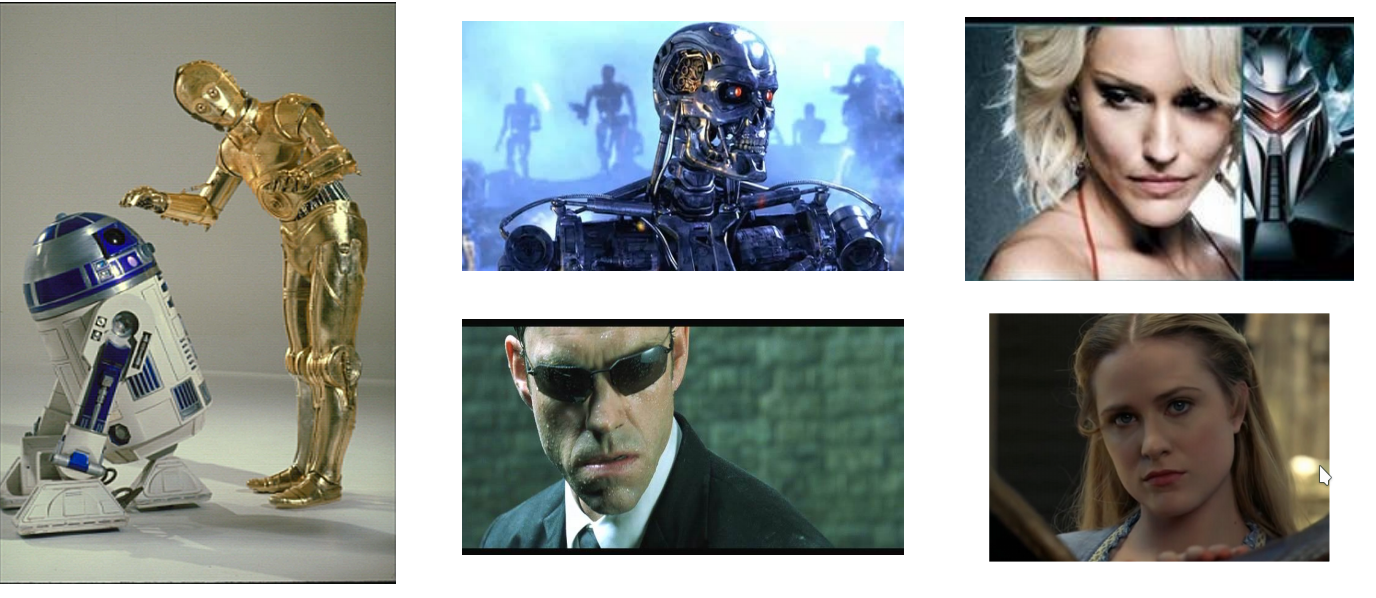
\includegraphics[width=1\textwidth]{img/ia1}
    \end{figure}

\end{frame}

\begin{frame}{¿Inteligencia Artificial?}

    \begin{columns}
        \begin{column}{0.32\textwidth}
            \begin{figure}[!h] 
                \centering
                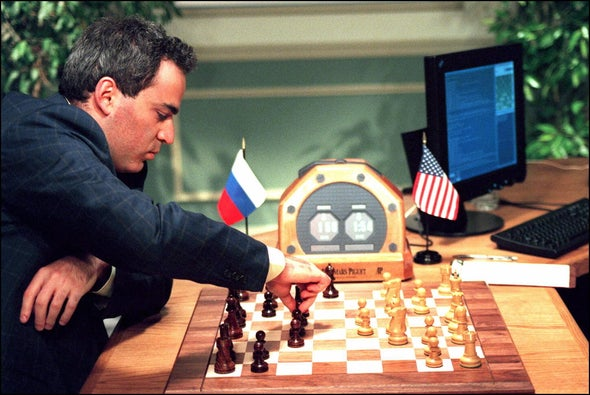
\includegraphics[width=1\textwidth]{img/deepblue}
            \end{figure}                
        \end{column}
        \begin{column}{0.32\textwidth}
            \begin{figure}[!h] 
                \centering
                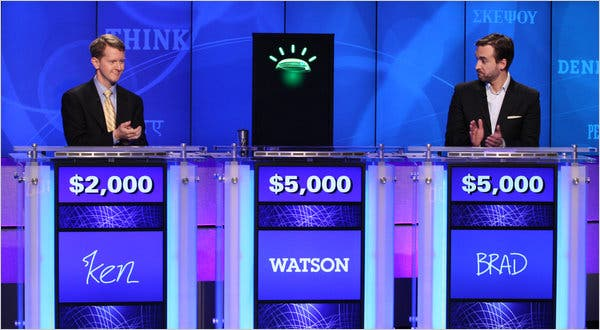
\includegraphics[width=1\textwidth]{img/watson}
            \end{figure}                
        \end{column}
        \begin{column}{0.32\textwidth}
            \begin{figure}[!h] 
                \centering
                
\includegraphics[width=1\textwidth]{img/alphago}
            \end{figure}                
        \end{column}
    \end{columns}
    
\end{frame}

\begin{frame}
    \frametitle{Enseñandole a una máquina}
    \begin{columns}
        \begin{column}{0.4\textwidth}
          \begin{itemize}
              \item Existen patrones dentro de los datos que producimos.
              \item El ser humano no es capaz de visualizar e identificar información oculta.
              \item A veces se necesita un \alert{modelo abstracto} que se aproxime a la naturaleza de los datos
          \end{itemize}
        \end{column}
        \begin{column}{0.6\textwidth}
          \begin{figure}[!h] 
            \centering
            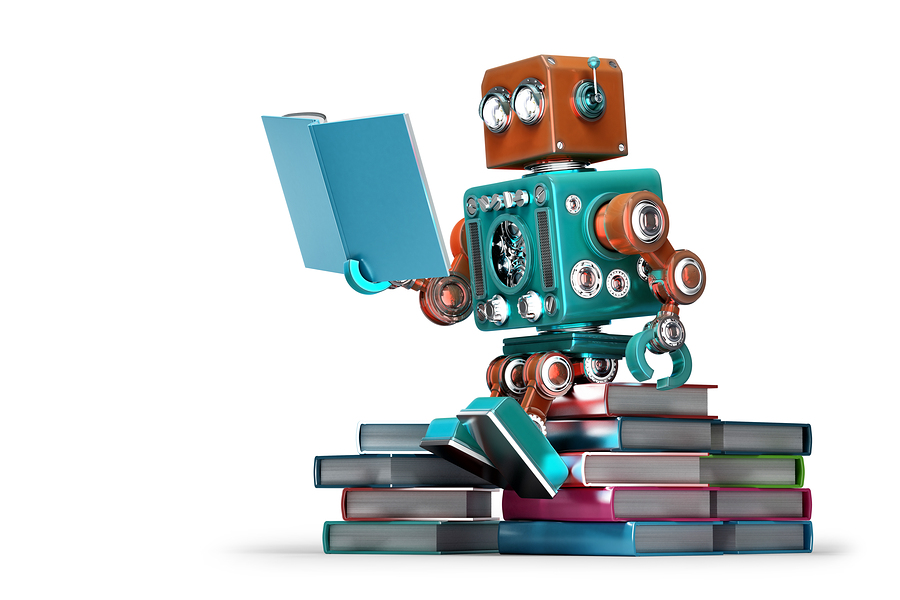
\includegraphics[width=1\textwidth]{img/robot1}
          \end{figure}  
        \end{column}
      \end{columns}

\end{frame}

\begin{frame}
    \frametitle{Tipos de Aprendizaje}
    \begin{columns}
        \begin{column}{0.5\textwidth}
          \begin{itemize}
              \item Aprendizaje Supervisado (Supervised Learning).
              \item Aprendizaje no supervisado (Unsupervised Learning).
              \item Aprendizaje por refuerzo (Reinforcement Learning).
          \end{itemize}
        \end{column}
        \begin{column}{0.5\textwidth}
          \begin{figure}[!h] 
            \centering
            
\includegraphics[width=1\textwidth]{img/robot2}
          \end{figure}  
        \end{column}
      \end{columns}

\end{frame}

\begin{frame}
    \frametitle{Un ejemplo...}
    \begin{figure}[!h] 
        \centering
        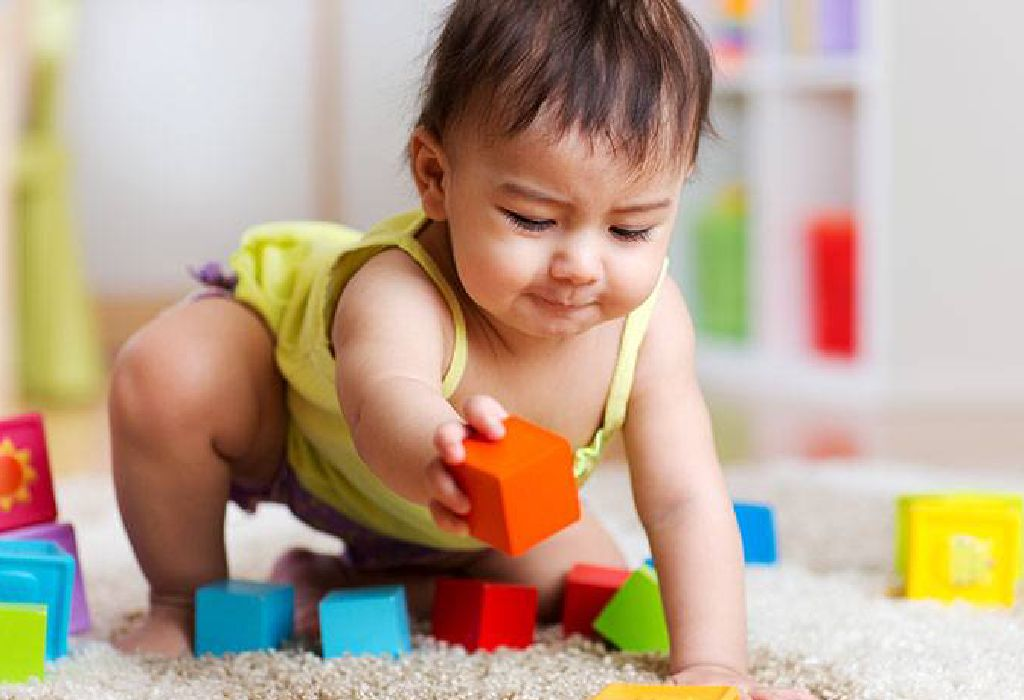
\includegraphics[width=1\textwidth]{img/bebe}
    \end{figure} 
\end{frame}

\begin{frame}
    \frametitle{Aprendizaje Supervisado}
    \begin{columns}
        \begin{column}{0.5\textwidth}
          \begin{itemize}
              \item Conjunto de datos etiquetados previamente.
              \item Existe una relación oculta entre entradas vs salidas: $x\Rightarrow y$
              \item Se pretende generalizar para nuevos ejemplos.
          \end{itemize}
        \end{column}
        \begin{column}{0.5\textwidth}
          \begin{figure}[!h] 
            \centering
            
\includegraphics[width=1\textwidth]{img/robot2}
          \end{figure}  
        \end{column}
      \end{columns}

\end{frame}

\begin{frame}
    \frametitle{Aprendizaje Supervisado}
    \begin{columns}
        \begin{column}{0.5\textwidth}
            Usualmente se tienen 2 tareas principales:
          \begin{itemize}
              \item Regresión.
              \item Clasificación.
          \end{itemize}
        \end{column}
        \begin{column}{0.5\textwidth}
          \begin{figure}[!h] 
            \centering
            
\includegraphics[width=1\textwidth]{img/robot2}
          \end{figure}  
        \end{column}
      \end{columns}

\end{frame}

\begin{frame}
    \frametitle{Otro ejemplo...}
    \begin{figure}[!h] 
        \centering
        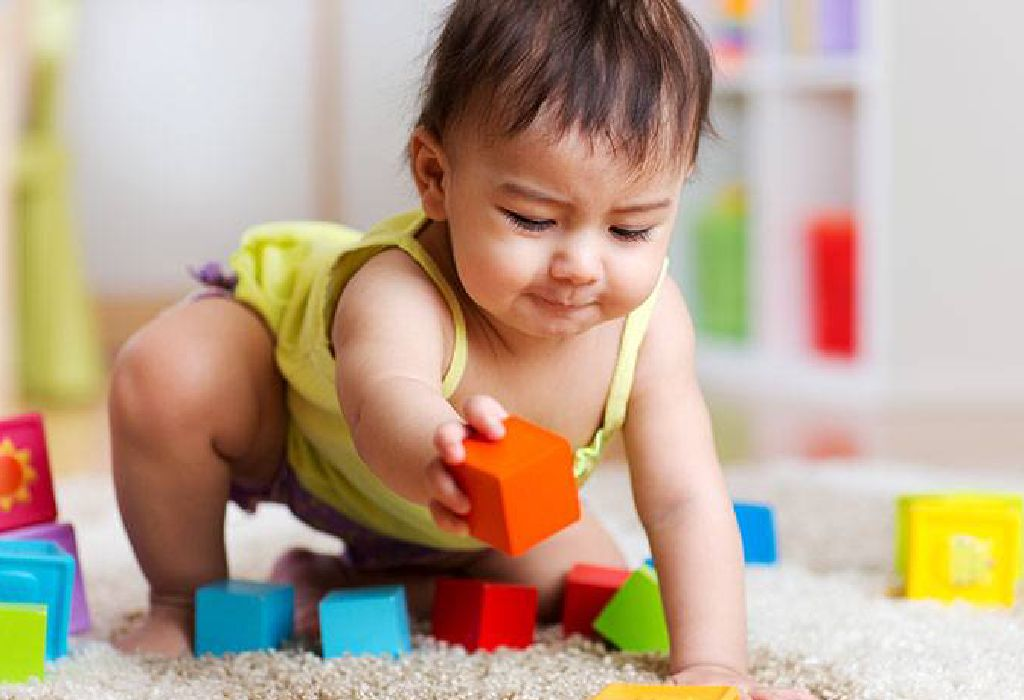
\includegraphics[width=1\textwidth]{img/bebe}
    \end{figure} 
\end{frame}

\begin{frame}
    \frametitle{Aprendizaje No Supervisado}
    \begin{columns}
        \begin{column}{0.5\textwidth}
          \begin{itemize}
              \item No existen etiquetas.
              \item Se intenta encontrar patrones ocultos en los datos.
              \item El algoritmo genera su propia representación de manera automática.
          \end{itemize}
        \end{column}
        \begin{column}{0.5\textwidth}
          \begin{figure}[!h] 
            \centering
            
\includegraphics[width=1\textwidth]{img/robot2}
          \end{figure}  
        \end{column}
      \end{columns}

\end{frame}

\begin{frame}
    \frametitle{Aprendizaje No Supervisado}
    \begin{columns}
        \begin{column}{0.5\textwidth}
            Se pueden encontrar las siguientes tareas:
          \begin{itemize}
              \item Clustering.
              \item Reducción de dimensionalidad.
              \item Detección de anomalías.
          \end{itemize}
        \end{column}
        \begin{column}{0.5\textwidth}
          \begin{figure}[!h] 
            \centering
            
\includegraphics[width=1\textwidth]{img/robot2}
          \end{figure}  
        \end{column}
      \end{columns}

\end{frame}

\begin{frame}
    \frametitle{Una vez más...}
    \begin{figure}[!h] 
        \centering
        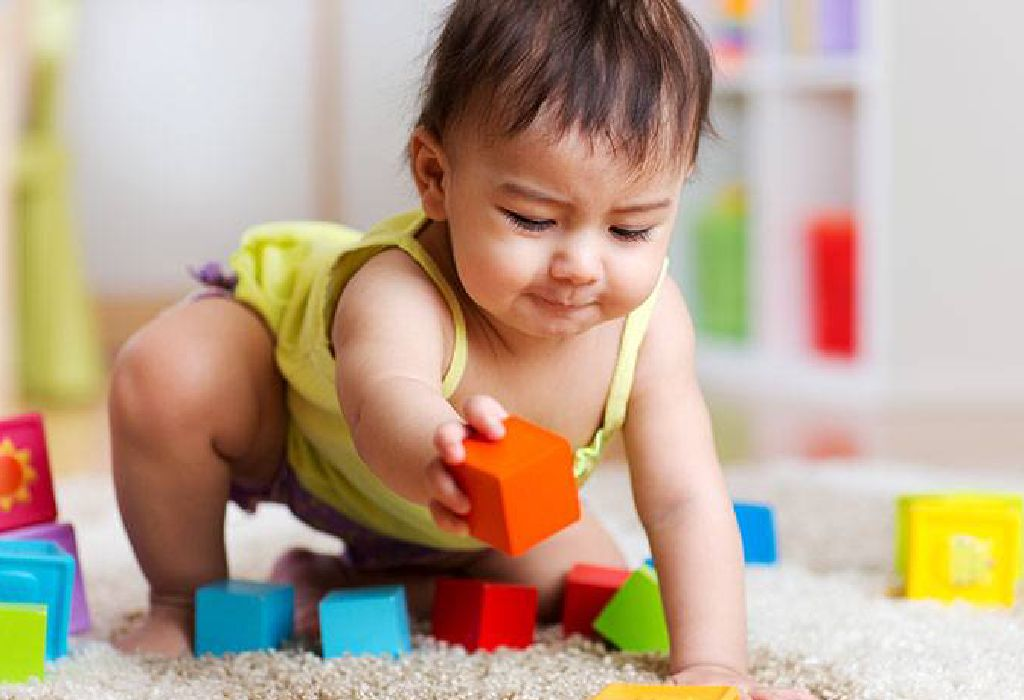
\includegraphics[width=1\textwidth]{img/bebe}
    \end{figure} 
\end{frame}

\begin{frame}
    \frametitle{Aprendizaje por Refuerzo}
    \begin{columns}
        \begin{column}{0.5\textwidth}
          \begin{itemize}
              \item Se basa en la interacción de un agente con su entorno.
              \item El agente modifica el estado del entorno.
              \item El entorno ofrece una recompensa.
              \item El agente debe maximizar la recompensa esperada.
          \end{itemize}
        \end{column}
        \begin{column}{0.5\textwidth}
          \begin{figure}[!h] 
            \centering
            
\includegraphics[width=1\textwidth]{img/robot2}
          \end{figure}  
        \end{column}
      \end{columns}

\end{frame}

\begin{frame}
    \frametitle{Aprendizaje por Refuerzo}
    \begin{columns}
        \begin{column}{0.5\textwidth}
            Se pueden encontrar las siguientes tareas:
          \begin{itemize}
              \item Robótica.
              \item Juegos.
              \item Optimización compleja.
              \item Control óptimo.
          \end{itemize}
        \end{column}
        \begin{column}{0.5\textwidth}
          \begin{figure}[!h] 
            \centering
            
\includegraphics[width=1\textwidth]{img/robot2}
          \end{figure}  
        \end{column}
      \end{columns}

\end{frame}

\begin{frame}
    \frametitle{En este curso}
    \begin{enumerate}
        \item Aprendizaje Supervisado.
            \begin{itemize}
                \item Regresión.
                \item Clasificación:
                    \begin{itemize}
                        \item Regresión Logística.
                        \item Naive Bayes.
                        \item SVM.
                        \item Decision trees.
                    \end{itemize}
            \end{itemize}
        \item Aprendizaje No Supervisado.
            \begin{itemize}
                \item Clustering.
                \item Reducción de dimensionalidad.
                \item Detección de anomalías.
            \end{itemize}
        \item Detalles de implementación.
            \begin{itemize}
                \item Análisis de Datasets.
                \item Evaluación de rendimiento.
                \item Aplicaciones.
            \end{itemize}
    \end{enumerate}
\end{frame}

\subsection{Aplicaciones}

\begin{frame}
    \frametitle{Lenguaje Natural}
    Tecnologías del habla:
    \begin{itemize}
        \item Reconocimiento automático de voz (ASR).
        \item Síntesis Texto a Voz (TTS).
        \item Sistemas de diálogo.
    \end{itemize}
    Procesamiento de lenguaje:
    \begin{itemize}
        \item Respuestas naturales.
        \item Traducción.
        \item Búsqueda en la web.
        \item Clasificación de textos.
    \end{itemize}
    
\end{frame}

\begin{frame}
    \frametitle{Visión}
    Pixeles $\Rightarrow$ Información / Decisión.

    \begin{itemize}
        \item Detección y reconocimiento de objetos.
        \item Segmentación Semántica.
        \item Entendimiento 3D.
    \end{itemize}
\end{frame}

\begin{frame}
    \frametitle{Robótica}
    Mitad Ingeniería mecánica, Mitad IA. El mundo real es mucho mas difícil que las simulaciones.

    \begin{itemize}
        \item Percepción.
        \item Planeamiento y control
        \item Monitoreo e interfaces humano - máquina.
    \end{itemize}
\end{frame}

\begin{frame}
    \frametitle{Juegos}
    \begin{itemize}
        \item 1997: Gary Kasparov cae ante DeepBlue.
        \item 2016: AlphaGo vence a Lee Sedol*.
        \item 2019: OpenAI Five vence a un equipo top de Dota 2*.
    \end{itemize}
\end{frame}


\begin{frame}
    \frametitle{Presencia de ML en nuestras vidas}
    El ML aplicada está presente a diario en nuestras vidas en las siguientes aplicaciones:

    \begin{itemize}
        \item Motores de búsqueda.
        \item Planeamiento de rutas.
        \item Logística e inventarios.
        \item Diagnósticos médicos.
        \item Servicios de soporte automatizado.
        \item Detección de Spam y fraude.
        \item Recomendaciones de productos.
        \item Traducción y procesamiento de textos.
        \pause
        \item ... Y mucho más!
    \end{itemize}
\end{frame}


{\setbeamercolor{palette primary}{fg=black, bg=yellow}
\begin{frame}[standout]
  Preguntas?
\end{frame}
}

\appendix

% \begin{frame}[fragile]{Backup slides}
%   Sometimes, it is useful to add slides at the end of your presentation to
%   refer to during audience questions.

%   The best way to do this is to include the \verb|appendixnumberbeamer|
%   package in your preamble and call \verb|\appendix| before your backup slides.

%   \themename will automatically turn off slide numbering and progress bars for
%   slides in the appendix.
% \end{frame}

% \begin{frame}[allowframebreaks]{Referencias}
% .
% \end{frame}

\end{document}
